\subsubsection{Finite State Machine of Course States in the Evaluation Process}
We used two methods to investigate the available artifact the FSM describing the states of courses in the evaluation process.
Firstly we executed the system on our machines.
We used test data to observe and test:

\begin{itemize}
    \item if every state of a course exists in the system
    \item if every transition exists as well as how and by whom the transition is initiated
    \item if states exist in the system that are not represented in the FSM
    \item if transitions are possible that are not represented in the FSM
\end{itemize} 

We found that some names of states differ between the Final State Machine and the system (\autoref{tab:state-names}).
\begin{table}[h]
    \centering
    \begin{tabular}{|l|l|}
        \hline
        FSM name                      & system name       \\ \hline \hline
        new                           & new               \\ \hline
        pending for lecturer approval & prepared          \\ \hline
        approved by lecturer          & lecturer approved \\ \hline
        approved by fsr               & approved          \\ \hline
        in evaluation                 & in evaluation     \\ \hline
        comment review pending        & evaluated         \\ \hline
        publication pending           & reviewed          \\ \hline
        published                     & published         \\ \hline
    \end{tabular}
    \caption{Comparing state names in FSM with state names in system}
    \label{tab:state-names}
\end{table}

Furthermore we found missing states and annotations (Figure \ref{fig:new-states}).

\begin{figure}[h]
    \centering
    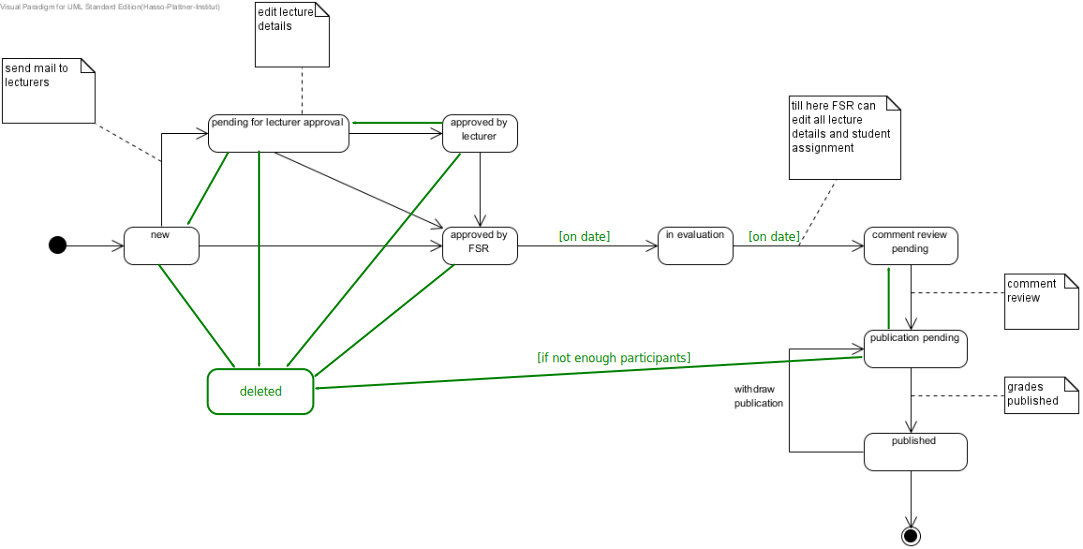
\includegraphics[width=\textwidth, keepaspectratio]{graphics/new_states_of_a_course}
    \caption{Updated FSM: Possible states of a course}
    \label{fig:new-states}
\end{figure}

Secondly, we were able to compare the FSM directly with the implementation found in \texttt{evap/evaluation/models.py} (Excerpt shown in \autoref{lst:states}).
A direct comparison is easy as there is a fsm package for the used webframework Django that was used to implement the FSM.

\lstinputlisting[language=Python, breaklines, columns=flexible, float, label=lst:states, caption=Excerpt of the implementation of course states.]{code/states.py}

Since the FSM was created several years ago, we suspect that either it was not complete from the start or it became outdated after updates to the code base.  
It is a pleasant suprise that there is a module that supports the direct implementation of FSMs since we learned that deriving FSMs is the hardest task if working with them.
%TODO reference to tests? Existing tests? New tests? No tests necessary because of fsm module?
